\chapter{Produto Educacional e Sequência Didática}

\section{Concepção do produto educacional}

A proposta educativa para o Ensino Médio envolve uma sequência didática e a criação de uma ferramenta web em português brasileiro que pode ser acessada, mesmo em redes com conectividade limitada. O recurso pode ser executado diretamente no navegador do computador, com a utilização de dados sintéticos, realizando o processamento da informação na máquina local do usuário. Esse fato torna o recurso muito interessante, pois não é necessário realizar login, as respostas não serão enviadas para servidor algum e não armazenará nenhum dado pessoal dos usuários. A única ação necessária para utilizar o recurso é abrir o projetor da sala ou os computadores disponíveis na mesma, facilitando ao professor de Computação a preservação do tempo de explicação e conversa em aula.

A proposta contém cinco módulos introdutórios a \textit{machine learning} (regressão linear, máquina de vetores de suporte - \textit{SVM}, \textit{k}-vizinhos mais próximos, árvore de decisão e \textit{k}-means) que não se limitam a apresentar um catálogo de comandos ou conteúdos soltos, mas colocam em confronto tarefas diferentes de previsão numérica e classificação, assim como a formação de grupos, para que os alunos possam notar o que muda de um módulo para o outro.

Cada módulo desenvolvido para a disciplina utiliza durante a aula uma própria camada matemática. Por exemplo, no módulo referente à regressão linear, os alunos precisam de todo o estudo realizado sobre a função e a linha de tendência para que consigam embasar a previsão e o cálculo dos erros ou resíduos. Já na \textit{SVM}, as classes são separadas pela fronteira traçada com sua margem. Já nos demais modelos utilizados nos módulos, como o \textit{k}-NN, os alunos precisam se debruçar sobre a distância entre os pontos. Para o \textit{k}-means, é preciso recalcular os centroides considerando a média, e para a árvore de decisão os alunos devem encadear condições. Assim, mesmo que haja mudança de nível de formalização entre eles, nada se perde, pois cada um segue o repertório dos alunos iniciantes e busca tornar visível, no gráfico ou na regra, uma relação discutível em sala.

No entanto, é interessante ressaltar que, além de estarem no mesmo site, cada atividade está interagindo e dialogando com as demais ao longo do percurso, por meio de perguntas semelhantes. Assim, antes de alterar qualquer controle na tela, os alunos devem conferir a origem do dado e a saída esperada para cada uma das atividades. Os resultados, assim como nas demais atividades apresentadas na sequência, variam em cada abordagem. Enquanto a regressão linear estima um número de maneira aproximada por meio de uma reta, a \textit{SVM} coloca uma fronteira entre os casos rotulados e considerados para treinamento do modelo. O \textit{k}-NN, por outro lado, consulta os vizinhos próximos de um ponto para determinar sua classe, a árvore segue regras condicionais e o \textit{k}-means busca agrupar pontos sem categorias prévias, apenas com base na proximidade entre eles.

Quando as mesmas questões reaparecem em cada módulo, os alunos acabam por comparar os modelos de maneira mais conceitual e não apenas como uma enumeração de termos técnicos. Além disso, o docente também consegue identificar se um determinado obstáculo está relacionado a uma ideia pontual ou se é devido às dificuldades inerentes à leitura de gráficos e dados presentes em todos os módulos. Conforme ilustra a Figura \ref{fig:plataforma-visao-geral}, a página inicial do sistema concentra a trilha das aulas, os cinco módulos e os materiais de apoio utilizados pelos estudantes durante o percurso.

\begin{figure}[H]
    \centering
    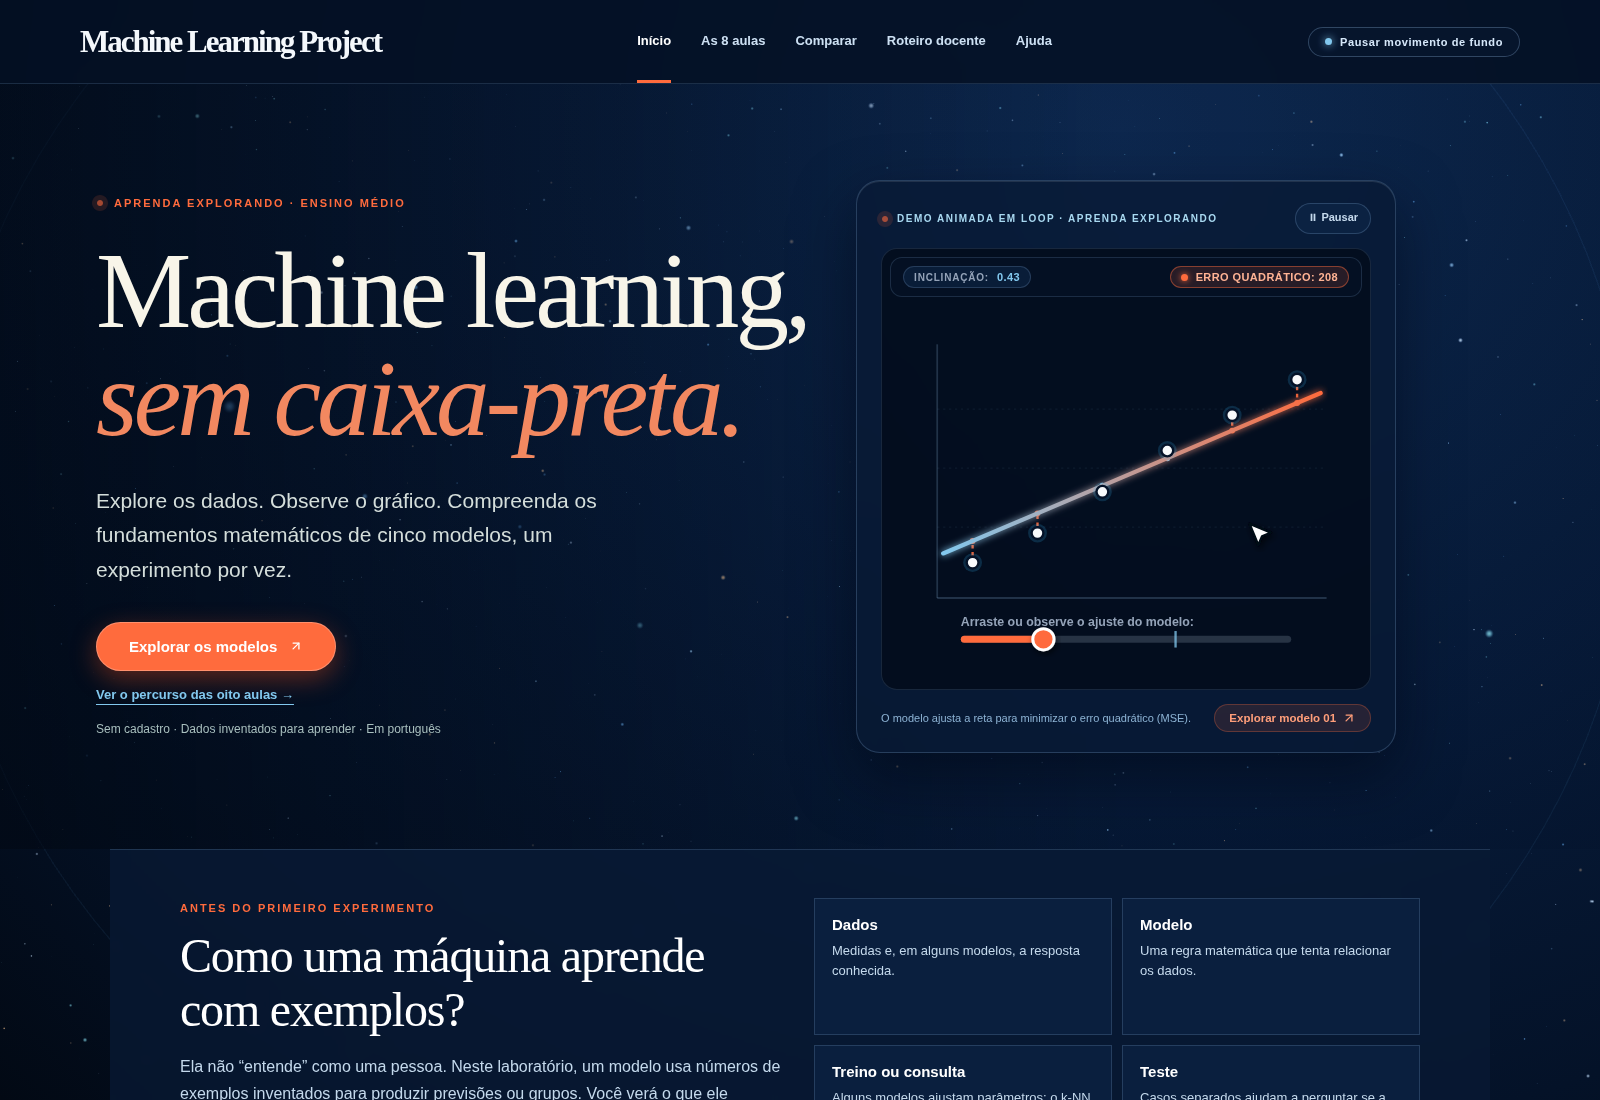
\includegraphics[width=0.94\textwidth]{figuras/plataforma-visao-geral.png}
    \caption{Visão geral da plataforma \textit{Machine Learning Project}.}
    \label{fig:plataforma-visao-geral}
    \source{Elaborado pelo autor (2026).}
\end{figure}

\section{Organização pedagógica da plataforma}

Em cada módulo, a aula parte de um cenário aplicado e abre a discussão sobre a procedência dos dados, para então perguntar ao aluno o que o algoritmo busca aprender nesse contexto. O estudante, antes de mexer nos controles presentes na tela, deve antecipar o que deve ocorrer. Em seguida, pode alterar os valores ou parâmetros e observar os efeitos tanto no gráfico, quanto na saída do modelo. Deve explicar o resultado e repetir essa sequência em toda a plataforma, para se consolidar o entendimento acerca de seu raciocínio em cada manipulação.

Um aspecto importante a ser considerado é que, ao mexer na reta e inclinar seu ângulo, a turma logo percebe a diferença entre o valor calculado e o dado real. Além disso, na tela da \textit{SVM}, quando o usuário puxa a fronteira para ficar mais próxima dos exemplos de uma classe específica, é um bom momento para o professor debater com os alunos o porquê da margem se encolher. A mesma ideia se repete em diferentes contextos, como quando os alunos trocam os vizinhos no \textit{k}-NN, ajustam as divisões da árvore ou mudam o lugar dos centroides no \textit{k}-means.

Para ilustrar o uso prático da plataforma, as Figuras \ref{fig:plataforma-regressao-linear} e \ref{fig:plataforma-svm} mostram dois módulos já abertos e em atividade. Na primeira interface, o estudante trabalha com a atividade de estimativa numérica apoiada na reta, enquanto que na segunda pode visualizar a divisa que separa os casos já rotulados. Em qualquer uma das duas telas, a tarefa consiste em que o aluno preveja o comportamento antes de tocar no controle e justifique posteriormente o que foi observado na prática.

\begin{figure}[H]
    \centering
    \begin{subfigure}[b]{0.48\textwidth}
        \centering
        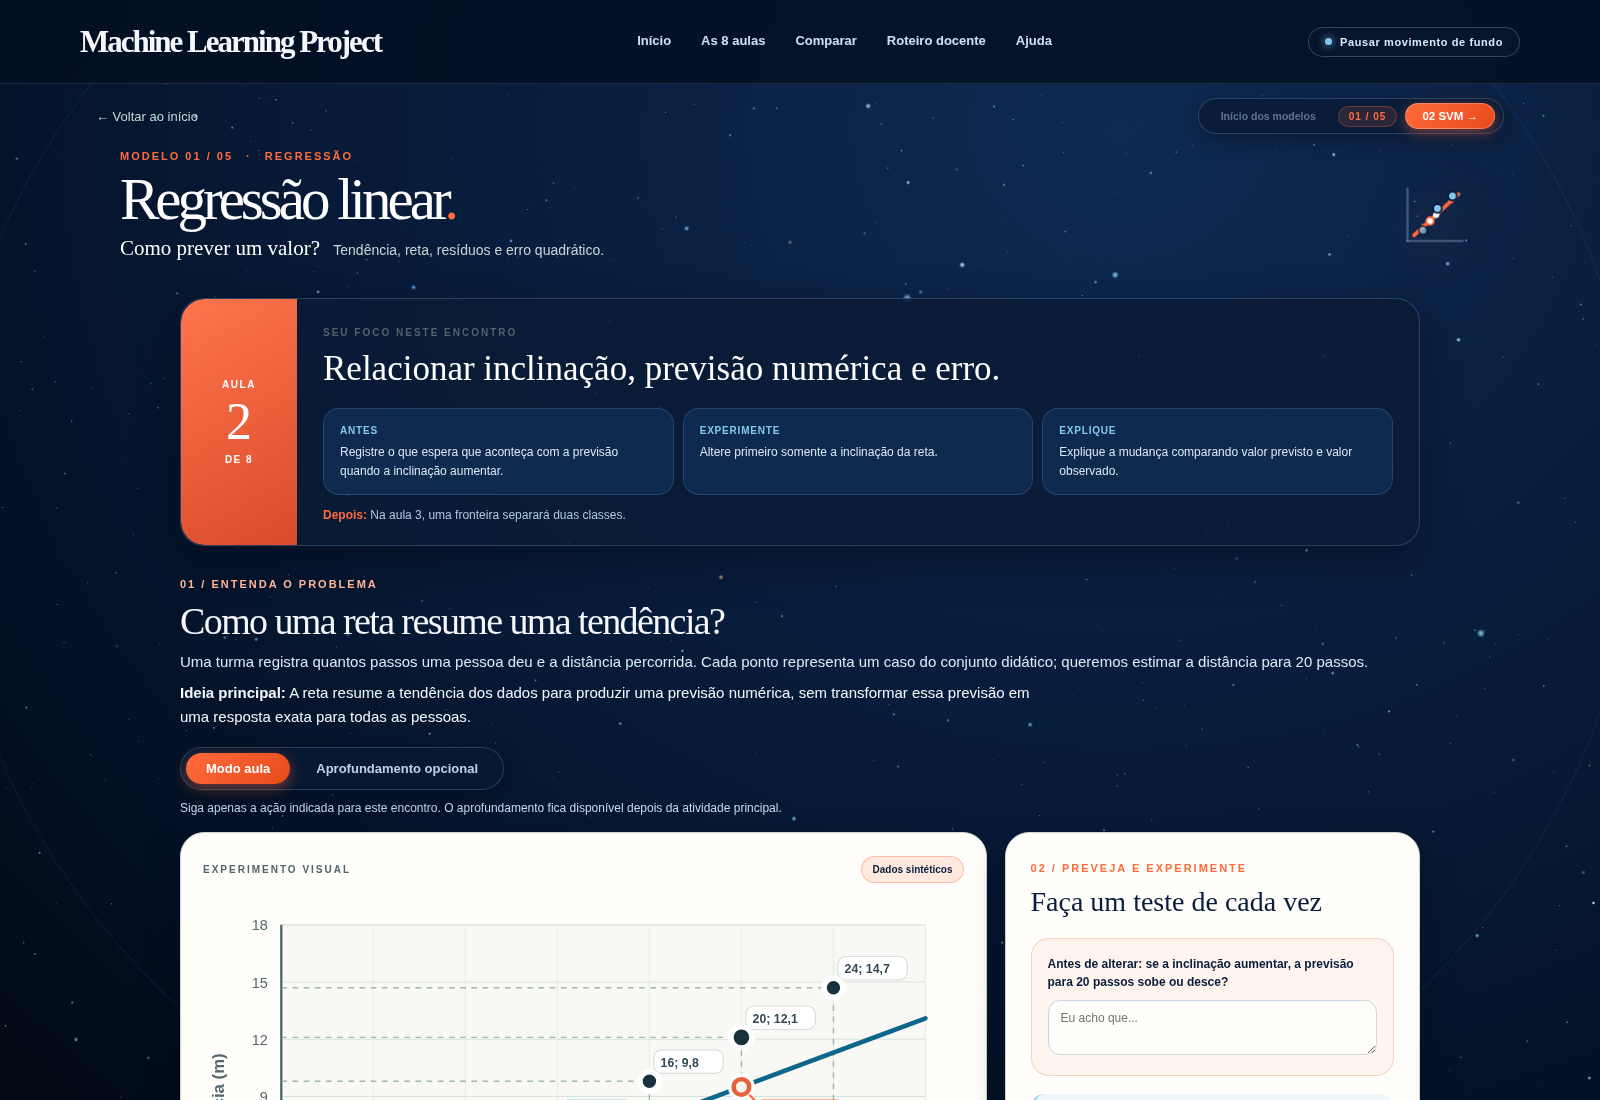
\includegraphics[width=\textwidth]{figuras/plataforma-regressao-linear.png}
        \caption{Módulo de regressão linear.}
        \label{fig:plataforma-regressao-linear}
    \end{subfigure}
    \hfill
    \begin{subfigure}[b]{0.48\textwidth}
        \centering
        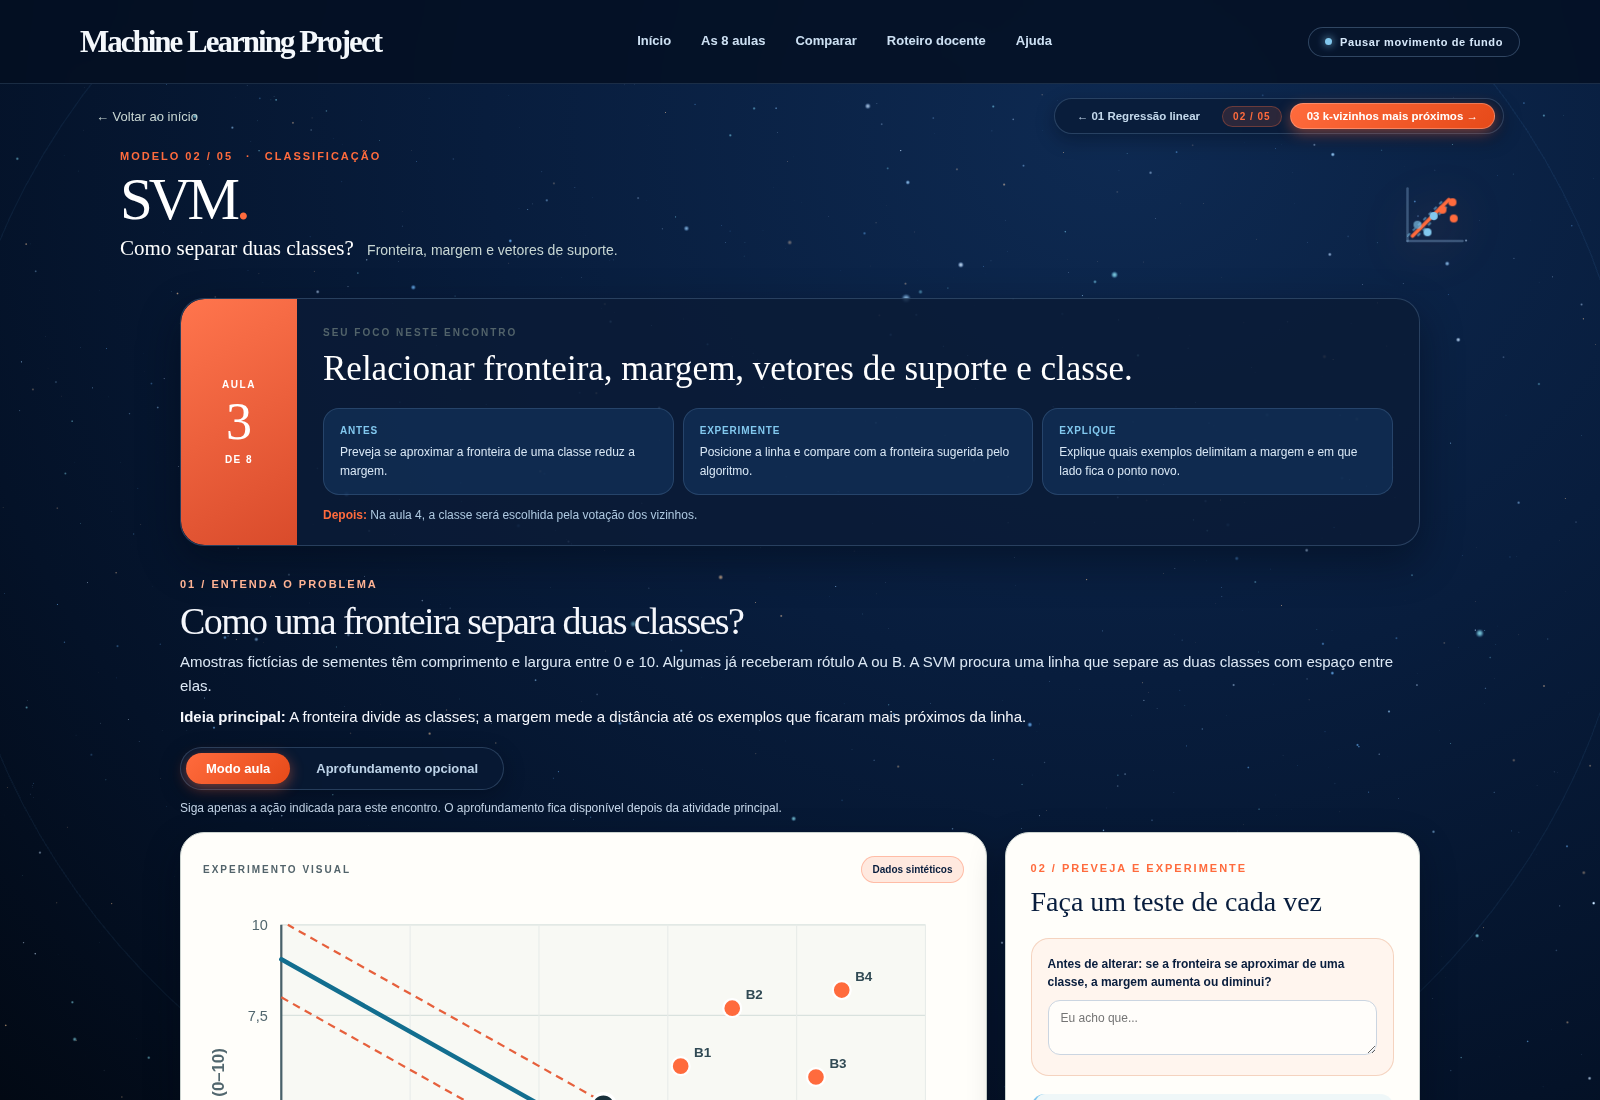
\includegraphics[width=\textwidth]{figuras/plataforma-svm.png}
        \caption{Módulo de \textit{SVM}.}
        \label{fig:plataforma-svm}
    \end{subfigure}
    \caption{Telas de módulos da plataforma interativa.}
    \source{Elaborado pelo autor (2026).}
\end{figure}

As aulas iniciais partirão de ferramentas de inteligência artificial que estão presentes no cotidiano dos estudantes e irão se aproximar rapidamente de um desafio mais concreto, por meio da visualização de dados. Durante as aulas os conceitos matemáticos serão construídos de acordo com a demanda, ao interpretarmos os gráficos e o critério de decisão exigido pela tarefa. Para que os alunos não se detenham somente no desenho gráfico para compreender o que estão fazendo, em todas as telas exibiremos quadros de dados e descrições textuais que deixarão a regra das telas claras. No protótipo disponível foi incluído o recurso de gráficos em 3D, porém esse será utilizado de forma opcional, não interferindo no conteúdo principal. Além disso, a interface também possibilita a operação por teclado e a opção de reduzir movimentos na tela.

\section{Cenários e dados dos experimentos}

Quase toda a base de dados utilizada nos experimentos será formada por informações sintéticas, sem aproveitamento de boletins de notas, anotações disciplinares de conduta ou qualquer informação pessoal dos estudantes. Como exceção pontual, na segunda aula os jovens poderão construir juntos uma tabela anônima com dados simples e voluntários, ou então medir objetos presentes na sala. Esse levantamento específico será realizado apenas para auxiliar a explicação didática em sala de aula e não fará parte do corpus da pesquisa.

Os cenários experimentais criados para a turma poderão ser modificados e receber acertos pontuais, após a verificação das condições locais de aplicação. Cada um apresenta uma maneira diferente de representação de dados para a prática da aprendizagem. Por exemplo, no caso da regressão linear os pontos de dados estão relacionados à quantidade de passos e distância percorrida, enquanto que na \textit{SVM} os pontos de dados são medidas simuladas de sementes para tentar distinguir entre duas classes. Já nos outros módulos, o \textit{k}-NN classifica comidas fictícias em doçura e acidez, o \textit{k}-means aproveita o mesmo par para formar grupos de pontos sem nenhuma categoria prévia e a árvore de decisão organiza os objetos em função da largura e altura.

Todos os contextos experimentais buscam deixar claro na interface do usuário o impacto de variar as entradas ou parâmetros, relacionando-os à Matemática correspondente ao ano letivo dos alunos. Para isso, antes da intervenção escolar, todo o conjunto de exemplos receberá uma revisão cuidadosa. O objetivo dessa conferência prévia é adequar o vocabulário das atividades e calibrar o tempo previsto de exploração às características reais da turma.

\section{Sequência didática provisória}

A sequência será aplicada em uma turma de Ensino Médio sob docência do pesquisador, já definida para o período de novembro de 2026. Serão oito encontros de cerca de cinquenta minutos, dentro do componente curricular acordado com a escola. O laboratório de informática dispõe de 20 computadores conectados à internet, e Chromebooks completarão o acesso individual quando necessário. A aplicação e a produção de dados dependerão das autorizações institucionais e éticas aplicáveis.

Todo encontro mantém a mesma estrutura, mesmo quando o modelo muda. A aula abre com uma situação ou pergunta que delimita o problema. Após registrar uma breve previsão inicial, cada estudante explora os controles de forma autônoma antes do debate coletivo e da síntese docente no fechamento. Essa rotina dá continuidade às aulas e integra a plataforma ao trabalho de construir e revisar hipóteses, evitando que o uso do site funcione como simples intervalo entre explicações.

O primeiro encontro serve para nivelar conceitos. Antes de qualquer modelo, a turma discute aplicações cotidianas de inteligência artificial. Depois distingue os dados e a regra do modelo, até apontar o que seria entregue ao sistema e o que se espera dele. O diagnóstico inicial é individual e acontece no começo desse encontro, antes da discussão, ou na aula anterior, conforme o tempo. Registra ideias de partida, sem antecipar os nomes técnicos que aparecem depois.

Do segundo ao sexto encontro entram, um por aula, os cinco módulos da plataforma, da regressão linear aos modelos de classificação e agrupamento. No segundo encontro, a organização da tabela da turma antecede a regressão linear. Cada aula retoma elementos anteriores para evitar que os modelos fiquem isolados em uma única experiência.

A regressão linear e a \textit{SVM} abrem a parte dos modelos supervisionados. Na linear, a turma identifica a linha de tendência no plano cartesiano para fazer previsões e compará-las aos valores observados, introduzindo a noção de erro. A \textit{SVM} retoma o uso de exemplos conhecidos e direciona o debate para a fronteira que separa classes e para a margem em torno dessa divisão. Essa sequência imediata permite contrastar a previsão de um valor numérico com a definição de uma categoria, mostrando que ambas dependem dos dados e das escolhas do modelo.

O \textit{k}-NN e a árvore de decisão são duas maneiras de chegar a uma classificação. No \textit{k}-NN, os estudantes observam o papel da distância e do número de vizinhos na votação; na árvore, acompanham regras condicionais e os caminhos até uma decisão. Comparar os dois afasta a ideia de que exista um algoritmo melhor que os outros. Ambos usam dados e regras, cada um à sua maneira, e entregam saídas que precisam ser lidas à luz do problema e dos exemplos disponíveis.

O \textit{k}-means traz uma mudança: os pontos não vêm com categorias dadas de antemão. A atividade volta à pergunta sobre o que se quer produzir com os dados e mostra que formar grupos por proximidade não é escolher uma classe conhecida. A atualização dos centroides e a observação da reorganização dos pontos poderão exigir mais tempo, pois a diferença entre agrupamento e classificação pode levar o professor a retomar a linguagem dos encontros anteriores. Uma síntese breve registra o modo como os cinco modelos articulam dados e regras para gerar uma saída, destacando o que muda conforme a finalidade de cada tarefa.

O sétimo encontro compara os cinco modelos. Diante de novas situações-problema, a turma justifica com base nos dados disponíveis se o caso exige previsão numérica, escolha de categoria ou formação de grupos. No oitavo encontro, cada estudante responde primeiro ao bloco de questões equivalentes às do diagnóstico e, na sequência, resolve um desafio de transferência inédito. Nessa etapa final, é preciso apontar os dados necessários para associar a tarefa a um modelo compatível, explicando o efeito esperado caso um parâmetro ou dado mude na regra.

O encontro comparativo recupera diferenças que possam ter ficado dispersas e prepara a transferência para o desafio final. Ao justificar que tipo de saída o problema demanda a partir dos dados disponíveis, o estudante considera a finalidade da tarefa antes de escolher o modelo. Enquanto o núcleo comparável permite examinar mudanças frente ao diagnóstico, o desafio de transferência mostra como os conceitos são mobilizados em novo contexto, entrando como evidência adicional sem equiparação direta com questões mais simples.

O trabalho na plataforma ocorrerá individualmente, com os computadores do laboratório e, conforme a disponibilidade confirmada no campo, Chromebooks para completar o acesso da turma. No segundo, no quarto e no sexto encontros, cada estudante também preencherá um registro curto antes e depois de explorar o site, cobrindo assim um exemplo de regressão, um de classificação e outro de agrupamento. Já o instrumento final será inteiramente individual. Caso o laboratório fique indisponível, o professor projetará os experimentos para a turma, preservando as pausas de previsão e explicação individual.

O roteiro preliminar dos oito encontros articula objetivos de aprendizagem e tempo previsto às ações de mediação com questões formativas, indicando ainda adaptações de infraestrutura e limites didáticos por módulo. Sem armazenamento de respostas digitadas no site, o corpus reunirá o diagnóstico inicial e o instrumento final completo, somados aos três registros individuais intermediários e às anotações docentes.

A versão do site usada no campo será conferida, antes da intervenção, com os recursos previstos na sequência. Se o cenário da plataforma tiver dados diferentes dos discutidos no roteiro da aula, a diferença será corrigida ou explicada aos estudantes; o mesmo vale para os textos de apoio e as representações matemáticas.

A pesquisa não pode analisar estudantes como se tivessem passado por uma sequência diferente do recurso usado. Essa conferência prática garante que a plataforma e os instrumentos avaliem exatamente o que foi trabalhado nas aulas.

\section{Materiais e limites do produto}

Além da plataforma, a aplicação contará com o diagnóstico inicial e três registros curtos de aula, somados às notas docentes e ao instrumento final com seu questionário de percepção. Nos registros intermediários, um campo recolhe a previsão prévia ao experimento e outro a explicação posterior. Já o questionário final consulta a turma sobre a clareza e o nível de dificuldade no manuseio do site, sem valer como evidência de aprendizagem.

O produto não comprova aprendizagem só por existir. Serve para que professor e estudantes discutam dados e parâmetros do modelo em sala.

A adequação didática do produto só poderá ser avaliada confrontando o planejamento com as condições reais do campo e as produções da turma, longe de constituir solução pronta para qualquer escola. Antes das aulas, um teste prático conferirá a abertura local do site nos computadores e a legibilidade da tela, checando ainda a resposta dos controles e a visibilidade no projetor. Caso algum equipamento falhe, o experimento seguirá projetado com pausas para registro individual.

A mudança de organização vai para o registro docente, porque a forma de acesso ao recurso pode alterar as interações observadas. Manter uma atividade pedagogicamente equivalente vale mais do que insistir em uma configuração técnica que a escola não consiga sustentar.

A mesma verificação confere se os estudantes compreendem os enunciados sem domínio prévio do jargão da área. Termos que vão de característica, vizinho e centroide até fronteira ou margem entram sempre acompanhados de exemplos visíveis e explicações situadas. Caso alguma pergunta gere dúvida recorrente, a revisão do enunciado ou da mediação será tratada como ajuste necessário ao produto, afastando a ideia de falha do estudante para remover barreiras linguísticas alheias ao conteúdo.

\section{Alinhamento curricular preliminar}

Uma matriz explicitará o vínculo da sequência com a Computação na Educação Básica, associando cada habilidade curricular ao seu objetivo de aprendizagem, bem como à atividade proposta e às evidências observáveis. A versão preliminar apoia-se nas referências do Ensino Médio voltadas aos fundamentos da inteligência artificial com suas potencialidades e limites, articulando a análise em ciência de dados ao uso de modelos computacionais simples de simulação e previsão. Esse recorte dialoga com as habilidades EM13CO10 a EM13CO12 previstas no anexo da Resolução CNE/CEB nº 1/2022 \cite{brasil2022computacao}. Embora a norma deixe de prescrever esses cinco algoritmos nominalmente, eles oferecem situações didáticas concretas para examinar os limites de cada regra na transformação de dados em resultados. A matriz indicará ainda conexões com a Matemática, mantendo a Computação como objeto principal. O recorte definitivo das habilidades dependerá da série e da disciplina definidas, respeitando o currículo da rede estadual e as condições do campo.
